\section{Analysis}
Firstly the data needs to be corrected because of random coincidences and misalignment of the setup. Random coincidence rate $\dot{R}$ is simply subtracted from the coincidence rate. In calculation of error of count rate, error of random coincidence is considered as well.
\begin{equation}
   \dot{R} = \SI{2.218 +- 0.061}{\per\s}
\end{equation}

It is thought to be acceptable to just use one random coincidence rate for all angles, since it has no angular dependence. Effects of misalignment on random coincidence need to be considered. That is why the random coincidence is to be subtracted first.

In figure.~\ref{fig:countRate}, one can see the trend in count rate of the mobile detector. This can be easily explained by source not being in the center of the setup. True data should be anti-proportional to count rates in figure.~\ref{fig:countRate}. Since measured angular correlation function is determined up to a proportional constant anyway, the normalization factor $\kappa$ is calculated by the fraction of count rate at smallest angle (this choice is arbitrary) and count rate at respective angle.
\begin{figure}[ht]
   \centering
   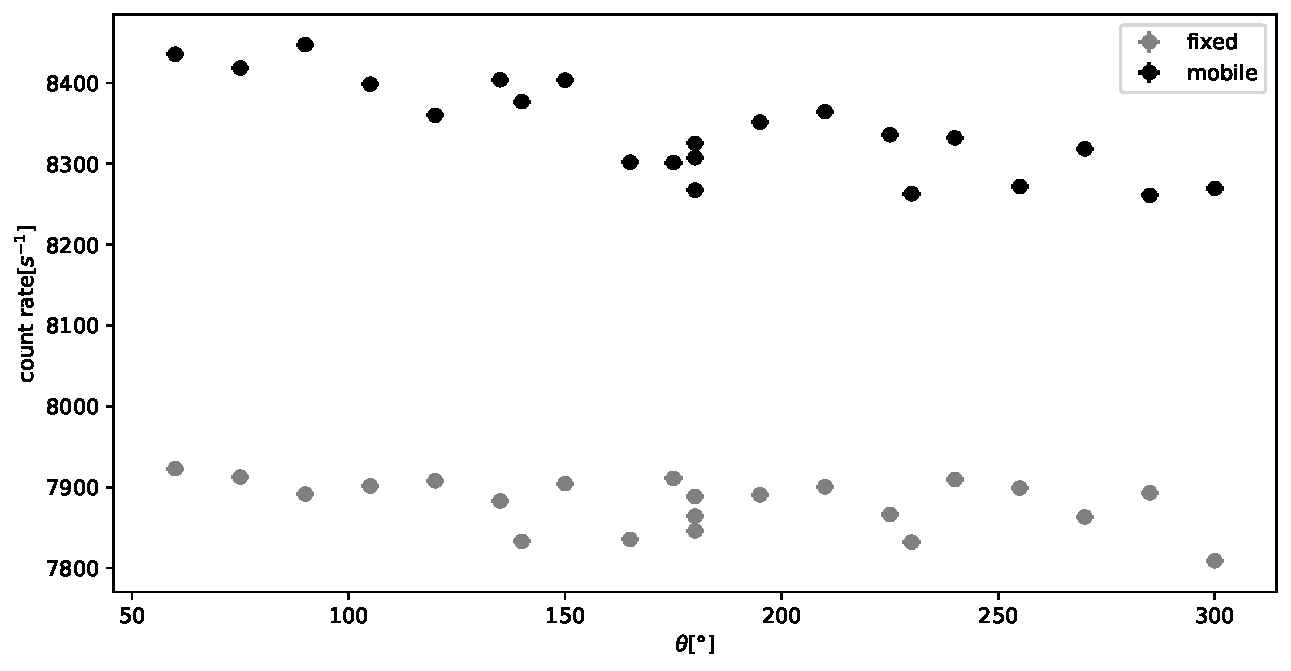
\includegraphics[width=0.8\linewidth]{./figs/countRate.pdf}
   \caption{Raw count rate}%
   \label{fig:countRate}
\end{figure}

Coincidence rates are normalized against the raw count rate with $\kappa$, in order to counter effects of misalignment. True coincidence rate $\dot{C}_{\text{true}}$ is calculated via
\begin{equation}
   \dot{C}_\text{true} = \kappa \cdot ( \dot{C}_\text{measured} - \dot{R})
\end{equation}

During experiment, the setup and its environment might (inevitably) change, i.e.~temperature. Measurements at $180°$ are repeated multiple times. Some variations are seen. This introduce (one source of) systematic error and will be included in the further analysis.
\begin{equation}
   \Delta \dot{C}_\text{sys} = \num{0.564}
\end{equation}

Data after these corrections are plotted in figure.~\ref{fig:angCor}. Vertical error bars include statistical error and systematic error. Error of angle is estimated to be about $2$ degrees.
\begin{figure}[ht]
   \centering
   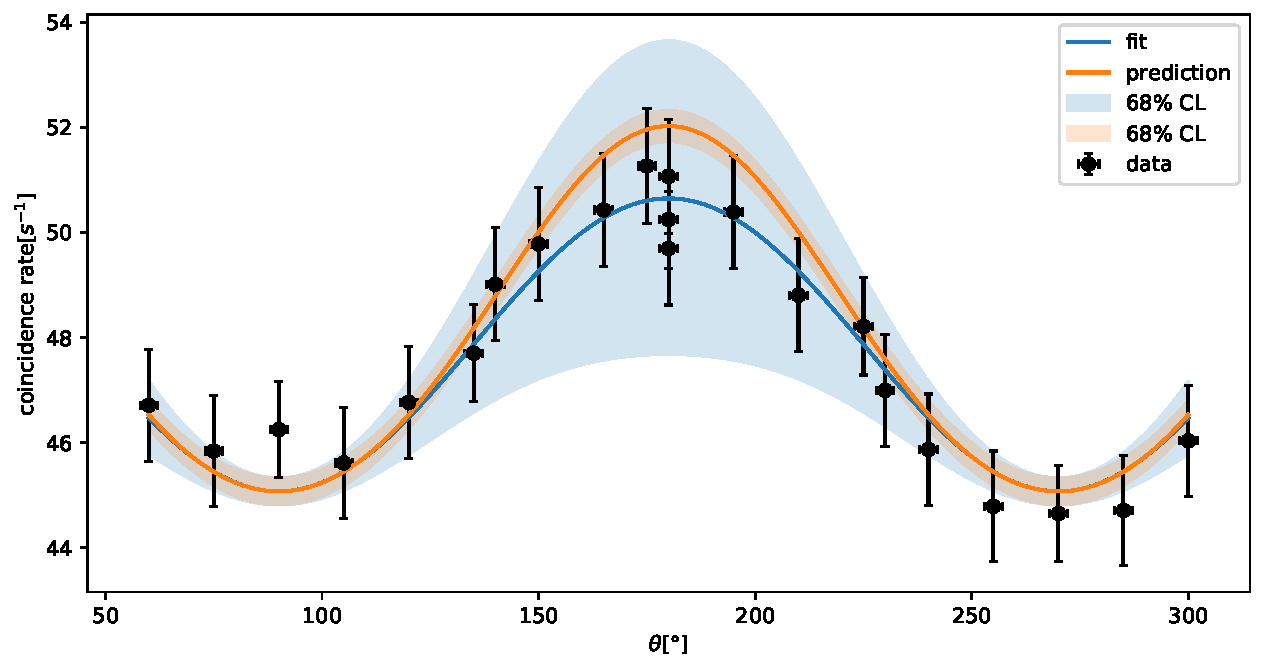
\includegraphics[width=0.8\linewidth]{./figs/angCor.pdf}
   \caption{Angular correlation with fit and prediction}%
   \label{fig:angCor}
\end{figure}

A least squares fit of data using function in the form of \eqref{math:fTheta} is carried out. Fitted function is drawn in blue in figure.~\ref{fig:angCor} alongside with its confidence intervals. Parameters are
\begin{align}
   \begin{split}
      A &= \num{45.072 +- 0.258}\\
      B &= \num{0.125 +- 0.031} \\
      C &= \num{-0.001 +- 0.029}
   \end{split}
\end{align}

Based on this value of $A$, we can plot the predicted function equation.~\eqref{math:pred}. Because of finite size of detector, prediction curve is "corrected" by factor $Q_k$ to correspond measured correlation curve. Values of $Q_k$ are taken from~\cite{siegbahn} with distance to source $h=\SI{5}{\cm}$. Energy of $\gamma$-radiation in experiment is between \SI{1}{\mega\eV} and \SI{1.5}{\mega\eV} and only photopeaks are relevant. For convenience, mean value of $Q_k$ of these two energies is used in calculation.
\begin{equation}
   Q_2 = \num{0.934},\; Q_4 = \num{0.792}
\end{equation}
Value of $A$ contains error, thus in figure.~\ref{fig:angCor} CLs are drawn around the prediction curve.

Although there are some deviation between prediction and fit curves, they are well within each other's $1\sigma$ range. Around $90$ and $270$ degrees, they match perfectly as expected. We have used $A$ value from fitting in drawing prediction curve. An independent determination of $A$ might be meaningful, but it is certainly beyond the scope of this experiment.

There is quite obvious asymmetry (with respect to $180$ degrees) present in the angular correlation. Ideally, this should not be in data, or at least after being corrected by considering misalignment. To better see the difference, data points are plotted in figure.~\ref{fig:angAsymm}. From this, we can see that the asymmetry can be well explained by the errors.
\begin{figure}[ht]
   \centering
   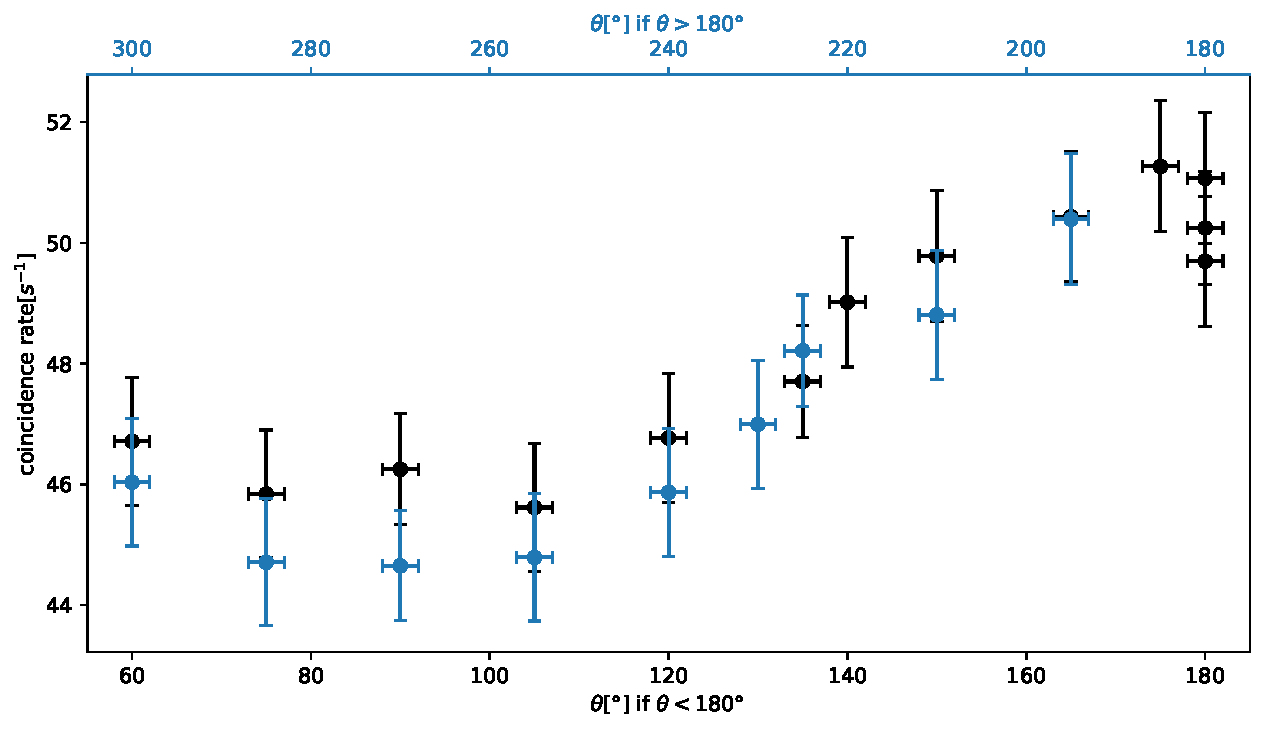
\includegraphics[width=0.8\linewidth]{./figs/angAsymm.pdf}
   \caption{Angular correlation to see asymmetry. Color of data points correspond to the color of axis to use.}%
   \label{fig:angAsymm}
\end{figure}
